\section{Results}

We have many parameters to take into account when we evaluate the performance of the broadcast and reduce operations. In order to make the analysis easier, we will fix some of them and vary the others.

\subsection{Broadcast}

By fixing the message size, we notice that the latency scales linearly with the number of processes.

As the size increases, Figure \ref{fig:broadcast_fixed_message_size_3}, a substantial positive performance is observed for the binary tree algorithm. And it takes advantage of the fact that the message is divided into smaller parts and sent to the processes in a binary tree fashion. The linear algorithm, on the other hand, has a constant performance, as it sends the message to all processes one by one.

The mapping does not seem to have a significant impact on the performance of the broadcast operation. The performance is almost the same for all the mappings.

It is interesting to notice, as show in Figure \ref{fig:broadcast_fixed_message_size_2}, that there is a ramp up in the latency when we reach 16 processes and 32 processes. It is not clear why this happens.

\begin{figure}[h!]
    \centering
    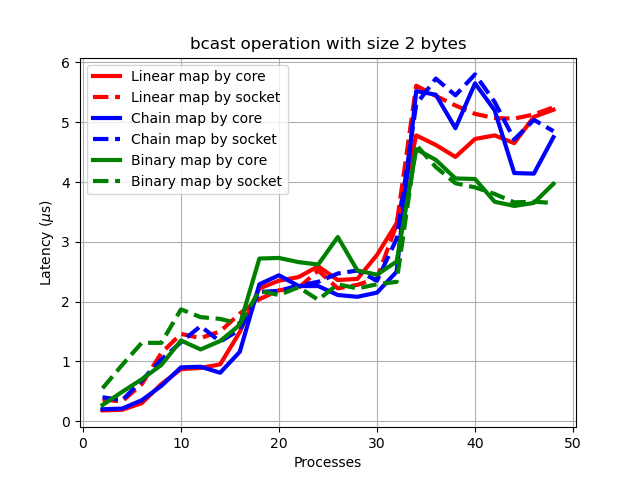
\includegraphics[width=0.8\textwidth]{../plots/bcast_fixedSize2.png}
    \caption{Broadcast 2 bytes fixed message size}
    \label{fig:broadcast_fixed_message_size_2}
\end{figure}

\begin{figure}[h!]
    \centering
    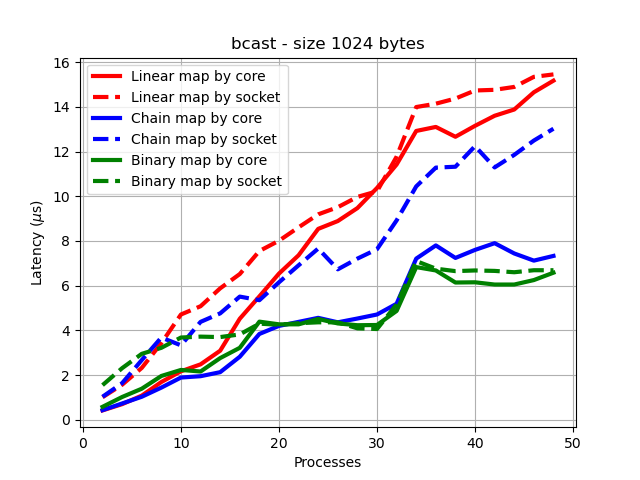
\includegraphics[width=0.8\textwidth]{../plots/bcast_fixedSize1024.png}
    \caption{Broadcast 1024 bytes fixed message size}
    \label{fig:broadcast_fixed_message_size_1024}
\end{figure}

\begin{figure}[h!]
    \centering
    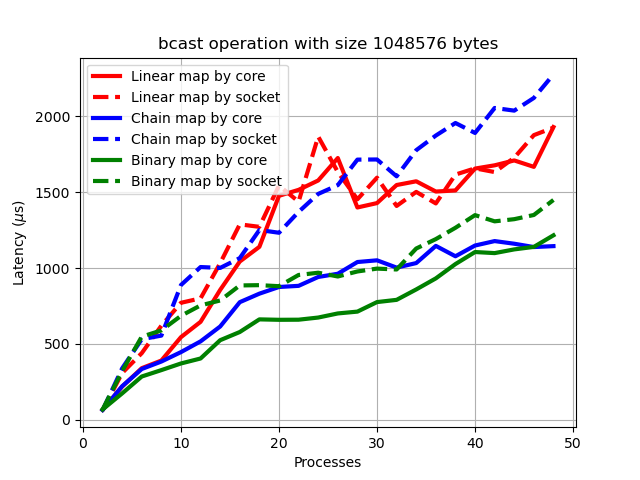
\includegraphics[width=0.8\textwidth]{../plots/bcast_fixedSize1048576.png}
    \caption{Broadcast 1 megabyte fixed message size}
    \label{fig:broadcast_fixed_message_size_1048576}
\end{figure}

Another kind of analysis that we can do is to fix the number of processes and vary the message size. In this case, we can see that the latency scales perfectly linearly with the message size. The binary tree algorithm has a better performance than the linear algorithm, as we can see in Figure \ref{fig:broadcast_fixed_processes_24}.

\begin{figure}[h!]
    \centering
    \includegraphics[width=0.8\textwidth]{../plots/bcast_fixedProcesses2.png}
    \caption{Broadcast with 2 processes}
    \label{fig:broadcast_fixed_processes_2}
\end{figure}

\begin{figure}[h!]
    \centering
    \includegraphics[width=0.8\textwidth]{../plots/bcast_fixedProcesses24.png}
    \caption{Broadcast with 24 processes}
    \label{fig:broadcast_fixed_processes_24}
\end{figure}

\begin{figure}[h!]
    \centering
    \includegraphics[width=0.8\textwidth]{../plots/bcast_fixedProcesses48.png}
    \caption{Broadcast with 48 processes}
    \label{fig:broadcast_fixed_processes_48}
\end{figure}



\subsection{Reduce}

Also in this case, by fixing the size of the message, the latency scales linearly with the number of processes. As noticed in the broadcast operation, the binary tree algorithm has a better performance than the linear algorithm.

As the message size increases, the mapping has no significant impact on the performance of the reduce operation performed by linear and binary algorithm. However, the chain algorithm performs significantly better using map by node policy for the processes, \ref{fig:reduce_fixed_message_size_1048576}.


\begin{figure}[h!]
    \centering
    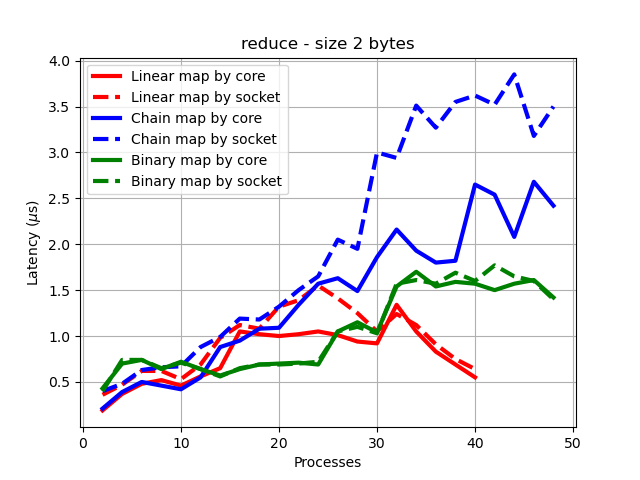
\includegraphics[width=0.8\textwidth]{../plots/reduce_fixedSize2.png}
    \caption{Reduce 2 bytes fixed message size}
    \label{fig:reduce_fixed_message_size_2}
\end{figure}

\begin{figure}[h!]
    \centering
    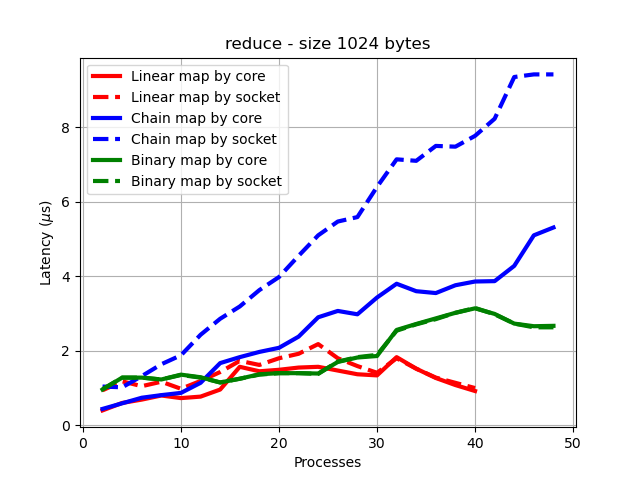
\includegraphics[width=0.8\textwidth]{../plots/reduce_fixedSize1024.png}
    \caption{Reduce 1024 bytes fixed message size}
    \label{fig:reduce_fixed_message_size_1024}
\end{figure}

\begin{figure}[h!]
    \centering
    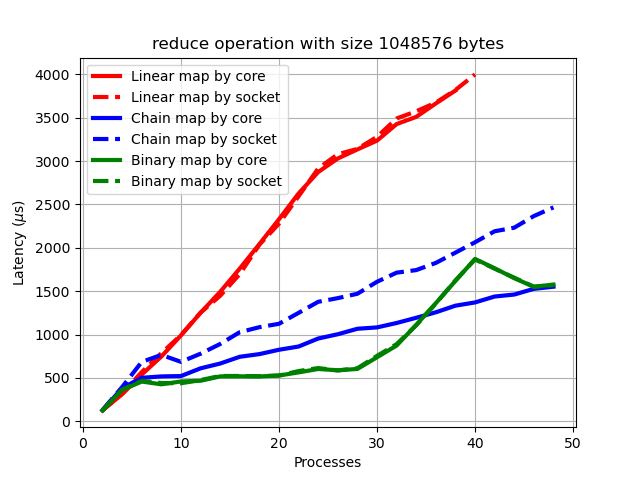
\includegraphics[width=0.8\textwidth]{../plots/reduce_fixedSize1048576.png}
    \caption{Reduce 1 megabyte fixed message size}
    \label{fig:reduce_fixed_message_size_1048576}
\end{figure}
